\section{Methodology}
\label{sec:method}

The measurements are performed in intervals of dimuon $\pt$ and absolute value of the rapidity ($|y|$). 
The term ``prompt'' refers to the $\jpsi$ or $\psiprime$ states --- hereafter called $\apsi$ to refer to either --- are produced 
from short-lived QCD decays, including feed-down from other charmonium states as long as they are also produced
from short-lived sources. If the decay chain producing a $\apsi$ state includes long-lived particles such as
$b$-hadrons, then such $\apsi$ mesons are labelled as ``non-prompt''. Using a simultaneous fit to the invariant mass of the dimuon and its ``pseudo-proper decay time'' 
(described below), prompt and non-prompt signal and background contributions can be extracted from the data.


The probability for the decay of a particle as a function of proper decay time $t$ follows an exponential distribution, 
$p(t) =  1/\tau_{B}\cdot e^{-t/\tau_{B}}$ where $\tau_{B}$ is the mean lifetime of the particle. For each decay, the proper decay time 
can be calculated as $t = L m/p$,
where $L$ is the distance between the particle production and decay vertices, $p$ is the momentum of the particle, and $m$ is its invariant mass.
As the non-prompt decays of $\apsi$ mesons do not fully reconstruct the $b$-hadron decay, the transverse momentum of the 
dimuon system and the reconstructed dimuon invariant mass are used to construct the
``pseudo-proper decay time'', $\tau = L_{xy} m(\mu\mu)/\pt(\mu\mu)$, where $L_{xy} \equiv \vec{L} \cdot \vec{\pt}(\mu\mu)/\pt(\mu\mu)$ 
is the signed projection of the distance of the dimuon decay vertex 
from the primary vertex, $\vec{L}$, onto its transverse momentum, $\vec{\pt}(\mu\mu)$.
This is a good approximation to using the parent $b$-hadron information when the $\psi$ and parent momenta are closely aligned, which is the case for the values of $\psi$
transverse momenta considered here, and  $\tau$
therefore can be used to distinguish statistically between the non-prompt and prompt processes (in which the latter are assumed to decay with vanishingly small lifetime).
If the event contains multiple primary vertices~\cite{ATLASdetector}, the primary vertex closest in $z$ to the dimuon decay vertex is selected.
The effect of selecting an incorrect vertex has been shown~\cite{BJpsiPhi} to have a negligible impact on the extraction of prompt and non-prompt contributions.
If any of the muons in the dimuon candidate contributes to the construction of the primary vertex, the corresponding tracks are removed and the vertex is refitted.


\subsection{Differential cross-section determination}
\label{sec:s:diff_xSecDet}

The differential dimuon prompt and non-prompt production cross-sections times branching ratio 
are measured separately for \jpsi\ and \psiprime\ mesons according to the equations:

\begin{equation}
\frac{\mathrm{d}^2\sigma(pp \rightarrow \psi)}{\mathrm{d}\pt\mathrm{d}y} \times \mathcal{B} (\psi \rightarrow \mu^+\mu^- ) = \frac{N_{\psi}^{\mathrm{p}}}{\Delta \pt \Delta y \times \int\mathcal{L} \mathrm{d}t}
\label{equ:xSecP}
\end{equation}
\begin{equation}
\frac{\mathrm{d}^2\sigma(pp \rightarrow b\bar{b} \rightarrow \psi)}{\mathrm{d}\pt\mathrm{d}y} \times \mathcal{B} (\psi \rightarrow \mu^+\mu^- ) = \frac{N_{\psi}^{\mathrm{np}}}{\Delta \pt \Delta y \times \int\mathcal{L} \mathrm{d}t}
\label{equ:xSecNP}
\end{equation}

\noindent where $\int\mathcal{L} dt$ is the integrated luminosity, $\Delta \pt $ and $ \Delta y$ are the interval sizes in terms of dimuon transverse momentum and
rapidity, respectively, and $N_{\psi}^{\mathrm{p(np)}}$ is the number of observed prompt (non-prompt) $\psi$ mesons in
the slice under study, corrected for acceptance, trigger and reconstruction efficiencies. 
The intervals in $\Delta y$ combine the data from negative and positive rapidities.
These differential cross-sections are determined separately for the \jpsi\ and \psiprime\ states.

The determination of the cross-sections proceeds in several steps. First, a weight is determined for each
selected dimuon candidate equal to the inverse of the total efficiency for each candidate. 
The total weight, $w_\mathrm{tot}$, for each dimuon candidate includes three factors: the fraction of produced $\psi \rightarrow \mu^+\mu^-$ decays with both
muons in the fiducial region $\pt (\mu) > 4$ \GeV\ and $|\eta(\mu)| <$ 2.3 (defined as acceptance, $\mathcal{A}$), the probability that a candidate
within the acceptance satisfies the offline reconstruction selection ($\epsilon_\mathrm{reco}$), and 
the probability that a reconstructed event satisfies the trigger selection 
($\epsilon_\mathrm{trig}$). The weight assigned to a given candidate when calculating the cross-sections is therefore  given by:

\begin{equation*}
w_{\mathrm{tot}}^{-1} = \mathcal{A} \cdot \epsilon_{\mathrm{reco}} \cdot \epsilon_{\mathrm{trig}}.
\end{equation*}

After the weight determination, an unbinned maximum-likelihood fit is performed to these weighted events in each ($\pt (\mu\mu), \ |y(\mu\mu)|$) interval using the 
dimuon invariant mass, $m(\mu\mu)$, and pseudo-proper decay time, $\tau(\mu\mu)$, observables. 
The fitted yields of $\jpsi \rightarrow \mu^+\mu^-$ and $\psiprime \rightarrow \mu^+\mu^-$ are determined separately for prompt and non-prompt processes. 
Finally, the differential cross-section times the  $\psi \rightarrow \mu^+\mu^-$ branching fraction is calculated for each
state by including the integrated luminosity and the $\pt$ and rapidity interval widths as shown in Eqs. (\ref{equ:xSecP}) and (\ref{equ:xSecNP}).


\subsection{Non-prompt fraction}
\label{sec:s:NPFDet}

The non-prompt fraction $f_{b}^{\psi}$ is defined as the number of non-prompt $\psi$ (produced
via the decay of a $b$-hadron) divided by the number of inclusively produced $\psi$ decaying to muon pairs after applying weighting corrections:

\begin{equation*}
f_{b}^{\psi} \equiv \frac{pp \rightarrow b + X \rightarrow \psi + X'}{pp \xrightarrow{\mathrm{Inclusive}} \psi + X'} = \frac{N^{\mathrm{np}}_{\psi}}{N^{\mathrm{np}}_{\psi} + N^{\mathrm{p}}_{\psi}}, 
\end{equation*}

\noindent where this fraction is determined separately for \jpsi\ and \psiprime. 
Determining the fraction from this ratio is advantageous since acceptance and efficiencies largely cancel and the systematic uncertainty is reduced.

\subsection{Ratio of \psiprime\ to \jpsi\ production in prompt and non-prompt production}
\label{sec:s:PNPRatioDet}

The ratio of \psiprime\ to \jpsi\ production, in their dimuon decay modes, is defined as:

\begin{equation*}
R^{\mathrm{p(np)}} =\frac{N^{\mathrm{p(np)}} _{\psi(2\mathrm{S})}}{N^{\mathrm{p(np)}} _{J/\psi}}
\end{equation*}

\noindent where $N_{\psi}^{\mathrm{p(np)}}$ is the number of prompt (non-prompt) \jpsi\ or \psiprime\ mesons decaying into a 
muon pair in an interval of $\pt$ and $y$, corrected for selection efficiencies and acceptance.

For the ratio measurements, similarly to the non-prompt fraction, the acceptance and efficiency corrections 
largely cancel, thus allowing a more precise measurement.
The theoretical uncertainties on such ratios are also smaller, as several dependencies, such as
parton distribution functions and $b$-hadron production spectra, largely cancel in the ratio.

\subsection{Acceptance}

The kinematic acceptance $\mathcal{A}$ for a $\psi \rightarrow \mu^+\mu^-$ decay with $\pt$ and $y$ is given by the 
probability that both muons pass the fiducial selection ($\pt(\mu)>4$ \GeV\ and $|\eta(\mu)|<2.3$).
This is calculated using generator-level simulations. 
Detector-level corrections, which are found to be small, are applied to the 
results and also considered as part of the systematic uncertainties. 

The acceptance $\mathcal{A}$ depends on five independent variables (the two muon momenta are constrained by the
$m(\mu\mu)$ mass condition), chosen as the $\pt$, $|y|$ and azimuthal angle $\phi$ of the $\psi$ meson in the laboratory frame,
and two angles
characterizing the $\psi \rightarrow \mu^+\mu^-$ decay, $\theta^{\star}$ and $\phi^{\star}$, described in detail in Ref. \cite{Faccioli:2010kd}.
The angle $\theta^{\star}$ is the angle between the direction of the positive-muon momentum in the $\psi$ rest frame
and the momentum of the $\psi$ in the laboratory frame, while $\phi^{\star}$ is defined as the angle between the dimuon 
production and decay planes in the laboratory frame. 
The $\psi$ production plane is defined by the momentum of the $\psi$ in the laboratory frame and the positive $z$-axis direction.
The distributions in $\theta^{\star}$ and $\phi^{\star}$ 
differ for various possible spin-alignment scenarios of the dimuon system.

The spin-alignment of the $\psi$ may vary depending on the production mechanism, which in turn affects the angular distribution of the dimuon decay.
Predictions of various theoretical models are quite contradictory, while the recent experimental measurements~\cite{Chatrchyan:2013cla} indicate that the angular dependence of $\jpsi$ and $\psiprime$
decays is consistent with being isotropic.  

The coefficients $\lambda_{\theta}, \lambda_{\phi}, \lambda_{\theta\phi}$ in
\begin{equation*}
\frac{\mathrm{d}^2N}{\mathrm{d}\cos\theta^{\star}\mathrm{d}\phi^{\star}} \propto 1 + \lambda_{\theta} \cos^2\theta^{\star} + \lambda_{\phi} \sin^2\theta^{\star}\cos2\phi^{\star} +  \lambda_{\theta\phi} \sin2\theta^{\star}\cos\phi^{\star}
\label{equ:acc}
\end{equation*}
\noindent are related to the spin-density matrix elements of the dimuon spin wave function. 

Since the polarization of the $\psi$ state may affect acceptance, seven extreme cases that lead to the largest possible variations of 
acceptance within the phase space of this measurement are identified.
These cases, described in Table~\ref{tab:spin}, are used to define a range in which the results may vary under any physically allowed spin-alignment assumptions.
The same technique has also been used in other measurements~\cite{Aad:2014fpa,ATLAS:2014ala,Aad2012dlq}.
This analysis adopts the isotropic distribution in both $\cos\theta^{\star}$ and $\phi^{\star}$ as  nominal,
and the variation of the results for a  number of extreme spin-alignment scenarios is studied and presented as sets of correction factors,
 detailed further in Appendix~\ref{sec:spincorrection}.
 
\begin{table}[htbp]
\begin{center}
\caption{Values of angular coefficients describing the considered spin-alignment scenarios.}
\vspace{2mm}
\begin{tabular}[h]{r|ccc}
\hline\hline
      & \multicolumn{3}{c}{Angular coefficients} \\ 
      & $\lambda_{\theta}$ & $\lambda_{\phi}$ & $\lambda_{\theta\phi}$ \\ \hline
Isotropic {\em (central value)}            & $0$ & $0$ & $0$ \\
Longitudinal         & $-1$ & $0$ & $0$ \\
Transverse positive  & $+1$ & $+1$ & $0$ \\
Transverse zero      & $+1$                & $0$ & $0$ \\
Transverse negative  & $+1$            & $-1$ & $0$ \\
Off-($\lambda_{\theta}$--$\lambda_{\phi}$)-plane positive   & $0$ & $0$ & $+0.5$ \\
Off-($\lambda_{\theta}$--$\lambda_{\phi}$)-plane negative   & $0$ & $0$ & $-0.5$ \\
\hline\hline
\end{tabular}
\label{tab:spin}
\end{center}
\end{table}


 
For each of the two mass-points (corresponding to the \jpsi\ and \psiprime\ masses), two-dimensional maps are produced
as a function of dimuon $\pt(\mu\mu)$ and $|y(\mu\mu)|$ for the set of spin-alignment hypotheses. 
Acceptance maps are defined within the range $8 < \pt(\mu\mu) < 110$ \GeV, $|y(\mu\mu)| < 2.0$, corresponding to the data
considered in the analysis. 
The map is defined by 100 slices in $|y(\mu\mu)|$ and 4400 in $\pt(\mu\mu)$, using 200k trials for each point, resulting in sufficiently high precision that the statistical uncertainty can be neglected.
Due to the contributions of background, and the detector resolution of the signal the acceptance for each candidate is determined from a linear interpolation of the two maps, which are generated for the \jpsi\ and \psiprime\ known masses, as a function of the reconstructed mass $m(\mu\mu)$.

Figure~\ref{fig:accMapUnpolBoth} shows the acceptance, projected in $\pt$ for all the spin-alignment hypotheses for the \jpsi\ meson.
The differences between the acceptance of the $\psiprime$ and $\jpsi$ meson, are independent of rapidity, except near $|y|\approx2$
at low $\pt$. Similarly, the only dependence on $\pt$ is found below $\pt\approx9$~\GeV.

\begin{figure}[ht]
  \begin{center}
    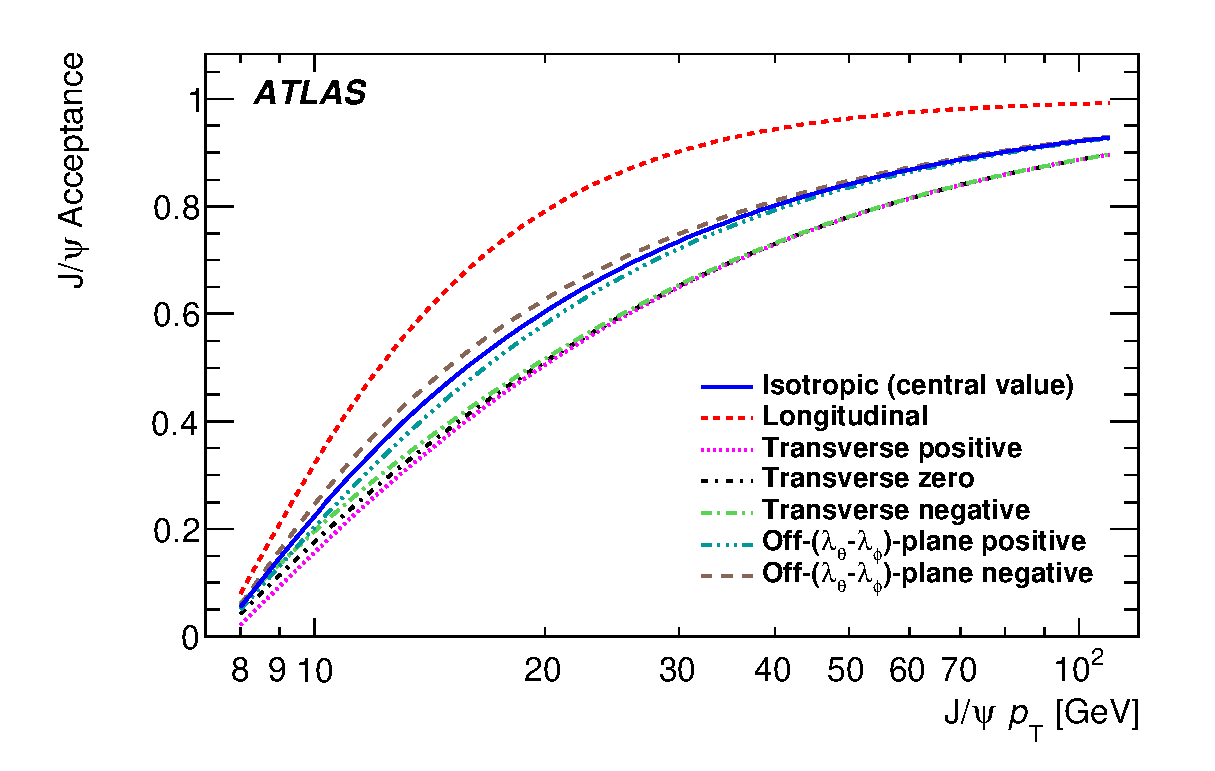
\includegraphics[width=0.8\textwidth]{c_JpsiAcc_All1D_logx.eps}
     \caption{Projections of the acceptance as a function of $\pt$ for the \jpsi\ meson for various spin-alignment hypotheses.}
     \label{fig:accMapUnpolBoth}
  \end{center}
\end{figure}



\subsection{Muon reconstruction and trigger efficiency determination}

\noindent The technique for correcting the 7~\TeV\ data for trigger and reconstruction inefficiencies is described in detail in Ref.~\cite{Aad:2014fpa,Aad2012dlq}.
For the 8~\TeV\ data, a similar technique is used, however different efficiency maps are required for each set of data, and the 8~\TeV\ corrections are detailed briefly below.

The single-muon reconstruction efficiency is determined from a tag-and-probe study in dimuon decays~\cite{Aad:2014kba}.
The efficiency map is calculated as a function of $\pt (\mu)$ and  $q\times \eta(\mu)$, where $q=\pm1$ is the electrical charge of the muon, expressed in units of $e$.

The trigger efficiency correction consists of two components. The first part represents the trigger efficiency for a 
single muon in intervals of $\pt (\mu)$ and $q\times \eta(\mu)$.
For the dimuon system there is a second correction to account for reductions in efficiency due to closely spaced
muons firing only a single RoI, 
vertex-quality cuts, and opposite-sign requirements.
This correction is performed in three rapidity intervals: 0--1.0, 1.0--1.2 and 1.2--2.3. The correction is a function of $\Delta R(\mu\mu)$ 
in the first two rapidity intervals and a function of $\Delta R(\mu\mu)$ and $|y(\mu\mu)|$ in the last interval.

The combination of the two components (single-muon efficiency map and dimuon corrections) is illustrated 
in Figure~\ref{fig:EFmu4DataJpsiTandPCmumupolyL2StarBMaxpt50} by plotting the average trigger-weight correction for the events in this analysis
in terms of $\pt(\mu\mu)$ and $|y(\mu\mu)|$.
The increased weight at low $\pt$ and $|y|\approx 1.25$ is caused by the geometrical acceptance of the muon trigger system and the turn-on threshold behaviour of the muon trigger. At high $\pt$ the weight is increased due to the reduced opening angle between the two muons.


\begin{figure} [!ht]
   \begin{center}
    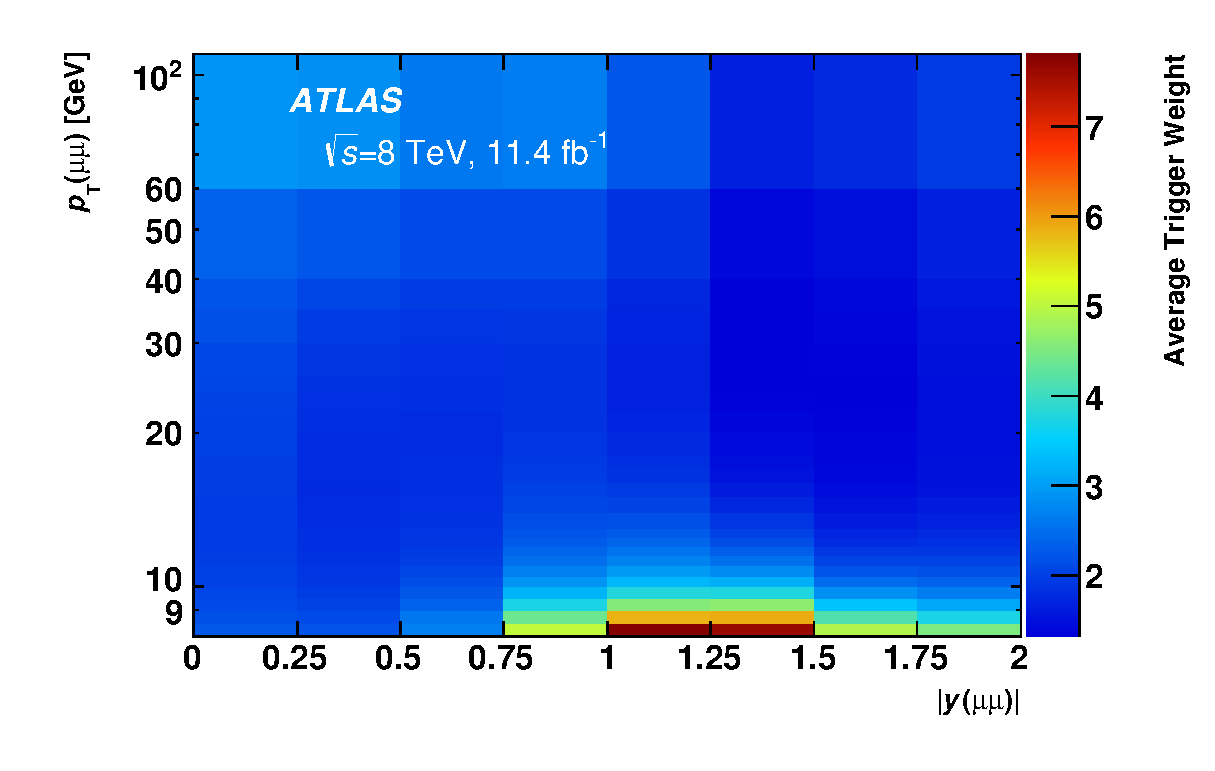
\includegraphics[scale=0.6]{averageTrigWeightMean.eps}
    \caption{Average dimuon trigger-weight in the intervals of $\pt (\mu\mu) $ and $ |y(\mu\mu)|$ studied in this set of measurements. 
    }
    \label{fig:EFmu4DataJpsiTandPCmumupolyL2StarBMaxpt50}
   \end{center}
\end{figure}


\subsection{Fitting technique}
\label{sec:method:fit}

The corrected prompt and non-prompt \jpsi\ and \psiprime\ signal yields are extracted from two-dimensional
weighted unbinned maximum-likelihood fits performed on the dimuon invariant mass ($m(\mu\mu)$)
and pseudo-proper decay time ($\tau(\mu\mu)$) in $(\pt (\mu\mu),|y(\mu\mu)|)$ intervals.
Each interval is fitted independently from all the others.
The probability density function (PDF) for each fit is defined as a normalized sum, 
where each term represents a specific signal or background contribution, with a physically motivated mass and $\tau$ dependence.
The PDF can be written in a compact form as
\begin{equation}
\label{eqn:pdf}
\mathrm{PDF}(m,\tau) = \sum_{i=1}^{7} \kappa_i f_i(m) \ \cdot h_i(\tau) \otimes R(\tau),
\end{equation}
where $\kappa_i$ represents the relative normalization of the $i^\mathrm{th}$ term of the seven considered signal and background contributions (such that $\sum_i \kappa_i = 1$), 
$f_i(m)$ is the mass-dependent term, and $\otimes$ represents the convolution of 
the $\tau$-dependent function $h_i(\tau)$ with the $\tau$ resolution term, $R(\tau)$. 
The latter is modelled by a double Gaussian distribution with both means fixed to zero and widths determined from the fit.

Table \ref{table:fitModel} lists the contributions to the overall PDF with the corresponding $f_i$ and
$h_i$ functions. Here $G_1$ and $G_2$ are Gaussian functions, $B_1$ and $B_2$ are Crystal Ball\footnote{The Crystal Ball function is given by:
\\$B(x;\alpha,n,\bar x,\sigma) = N \cdot \begin{cases} \exp\left(- \frac{(x - \bar x)^2}{2 \sigma^2}\right), & \mbox{for }\frac{x - \bar x}{\sigma} > -\alpha \\
 A \cdot \left(A' - \frac{x - \bar x}{\sigma}\right)^{-n}, & \mbox{for }\frac{x - \bar x}{\sigma} \leqslant -\alpha \end{cases}$ \\where $A = \left(\frac{n}{\left| \alpha \right|}\right)^n \cdot \exp\left(- \frac {\left| \alpha \right|^2}{2}\right),
A' = \frac{n}{\left| \alpha \right|}  - \left| \alpha \right|$}
distributions~\cite{CB1}, 
while F is a uniform distribution and $C_1$ a first-order Chebyshev polynomial. 
The exponential functions $E_1$, $E_2$, $E_3$, $E_4$ and $E_5$
have different decay constants, where $E_5(|\tau|)$ is a double-sided exponential with the same decay constant on
either side of $\tau = 0$. The parameter $\omega$ represents the fractional contribution 
of the $B$ and $G$ mass signal functions, while $\delta (\tau)$, the Dirac delta function,  
is used to represent the pseudo-proper decay time distribution of the prompt candidates.

\begin{table}[h!]
  \centering
  \caption{Description of the fit model PDF in Eq.~\ref{eqn:pdf}. Components of the probability density function used to extract the prompt (P) and
non-prompt (NP) contributions for \jpsi\ and \psiprime\ signal and the P, NP, and incoherent or mis-reconstructed  background (Bkg) contributions.}
    \begin{tabular}{ l  c  c  c  c  }
      \hline \hline
      $i$ & Type & Source & $f_i(m)$ & $h_i(\tau)$ \\ \hline \hline
      1 & \jpsi\     & P     & $\omega B_1(m) + (1-\omega) G_1(m)$   & $\delta (\tau)$ \\
      2 & \jpsi\     & NP    & $\omega B_1(m) + (1-\omega) G_1(m)$   & $ E_1(\tau)$ \\
      3 & \psiprime\    & P    & $\omega B_2(m) + (1-\omega) G_2(m)$   & $\delta (\tau)$ \\
      4 & \psiprime\   & NP    & $\omega B_2(m) + (1-\omega) G_2(m)$   & $E_2(\tau)$ \\ \hline
      5 & Bkg          & P     & $ F$     & $\delta (\tau)$ \\
      6 & Bkg          & NP    & $ C_1(m)$    & $E_3 (\tau)$ \\ 
      7 & Bkg          & NP    & $ E_4(m)$   & $E_5 (|\tau|)$ \\
      \hline  
    \end{tabular}
  \label{table:fitModel}
\end{table}

In order to make the fitting procedure more robust and to reduce the number of free parameters, a number of component terms share common parameters, 
which led to 22 free parameters per interval.
In detail, the signal mass models are described by the sum of a Crystal Ball shape ($B$) and a Gaussian shape ($G$). For each
of \jpsi\ and \psiprime, the $B$ and $G$ share a common mean, and freely determined widths, 
with the ratio of the $B$ and $G$ widths common to \jpsi\ and \psiprime.
The $B$ parameters $\alpha$, and $n$, describing the transition point of the low-edge from a Gaussian to a power-law 
shape, and the shape of the tail, respectively, are fixed, and variations are considered as part of the fit model
systematic uncertainties.
The width of $G$ for \psiprime\ is set to the width for \jpsi\ multiplied by a free parameter scaling term.
The relative fraction of $B$ and $G$ is left floating, but common to \jpsi\ and \psiprime.

The non-prompt signal decay shapes ($E_1$,$E_2$) are described by an exponential function (for positive $\tau$ only) convolved with a
double Gaussian function, $R(\tau)$ describing the pseudo-proper decay time resolution for the non-prompt component, 
and the same Gaussian response functions to
describe the prompt contributions. 
Each Gaussian resolution component has its mean fixed at $\tau$ = 0 and a free width.
The decay constants of the \jpsi\ and \psiprime\ are separate free parameters in the fit.

The background contributions are described by a prompt and non-prompt component, as well as a double-sided exponential function
convolved with a double Gaussian function describing mis-reconstructed or non-coherent dimuon pairs. 
The same resolution function as in signal is used to describe the background. For the non-resonant mass
parameterizations, the non-prompt contribution is modelled by a first-order Chebyshev polynomial. The prompt mass
contribution follows a flat distribution and the double-sided background uses an exponential function.
Variations of this fit model are considered as systematic uncertainties.

The following quantities are extracted directly from the fit in each interval:
the fraction of events that are signal (prompt or non-prompt \jpsi\ or \psiprime); the fraction of signal events that are prompt;
the fraction of prompt signal that is \psiprime; and the fraction of non-prompt signal that is \psiprime. From these
parameters, and the weighted sum of events, all measured values are calculated.


For $7$~\TeV\ data, 168 fits are performed across the range of $8<\pt<100$~\GeV\ ($8<\pt<60$~\GeV) for $\jpsi$ ($\psiprime$) and $0<|y|<2$.
For $8$~\TeV\ data, 172 fits are performed across the range of $8<\pt<110$~\GeV\ and $0<|y|<2$,
excluding the area where $\pt$ is less than 10 \GeV\ and simultaneously $|y|$ is
greater than 0.75. This region is excluded due to a steeply changing low trigger efficiency 
causing large systematic uncertainties in the measured cross-section.

Figure~\ref{fig:fitprojmain} shows the fit results for one of the intervals considered in the analysis with the overall and individual contributions superimposed on the data, and projected onto the invariant mass and pseudo-proper decay time distributions for  $7$~\TeV\ data.
In Figure~\ref{fig:fitprojmainVIII} the fit results are shown for one high-$\pt$ interval of $8$~\TeV\  data.

\begin{figure} [!ht]
  \begin{center} 
   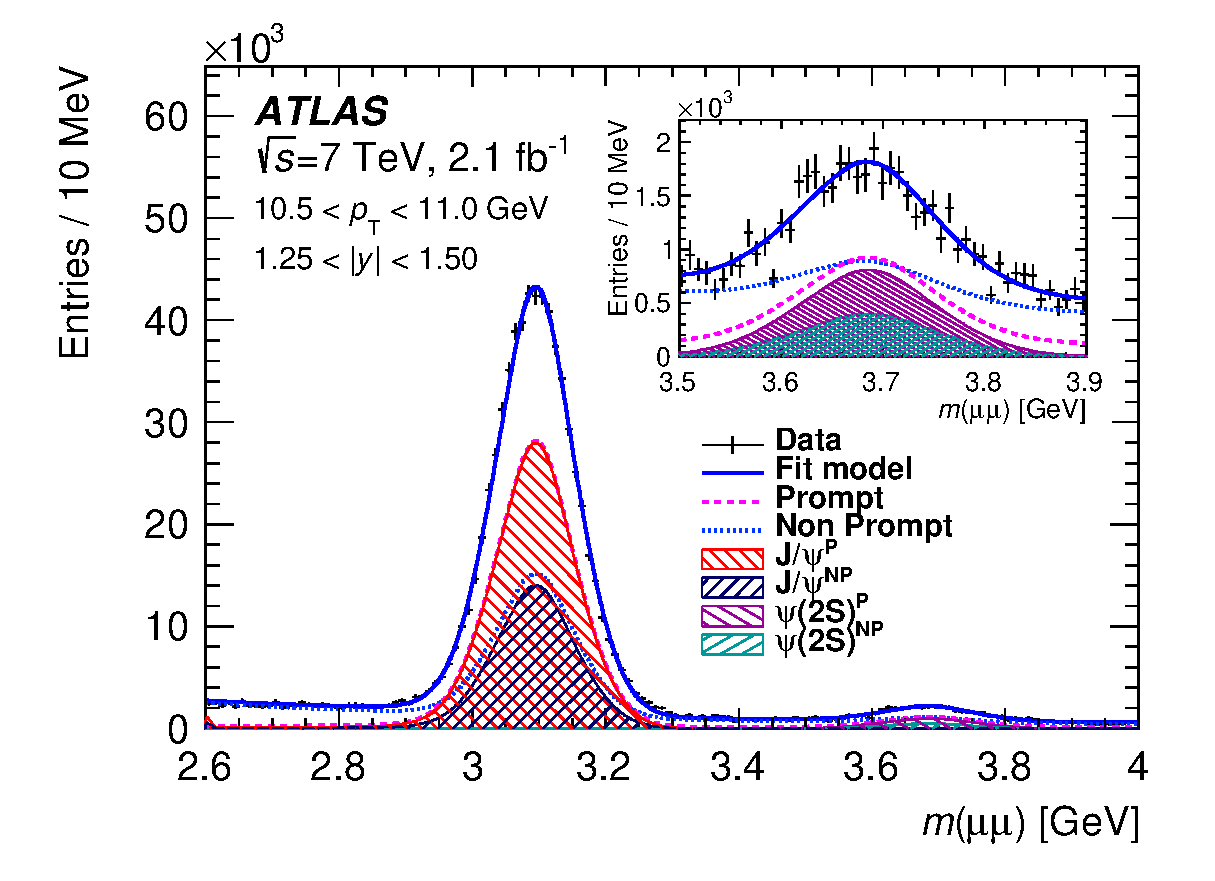
\includegraphics[width=0.51\textwidth]{figures/c_c_Mass_5_5.eps}
   \hspace{-0.55cm}
   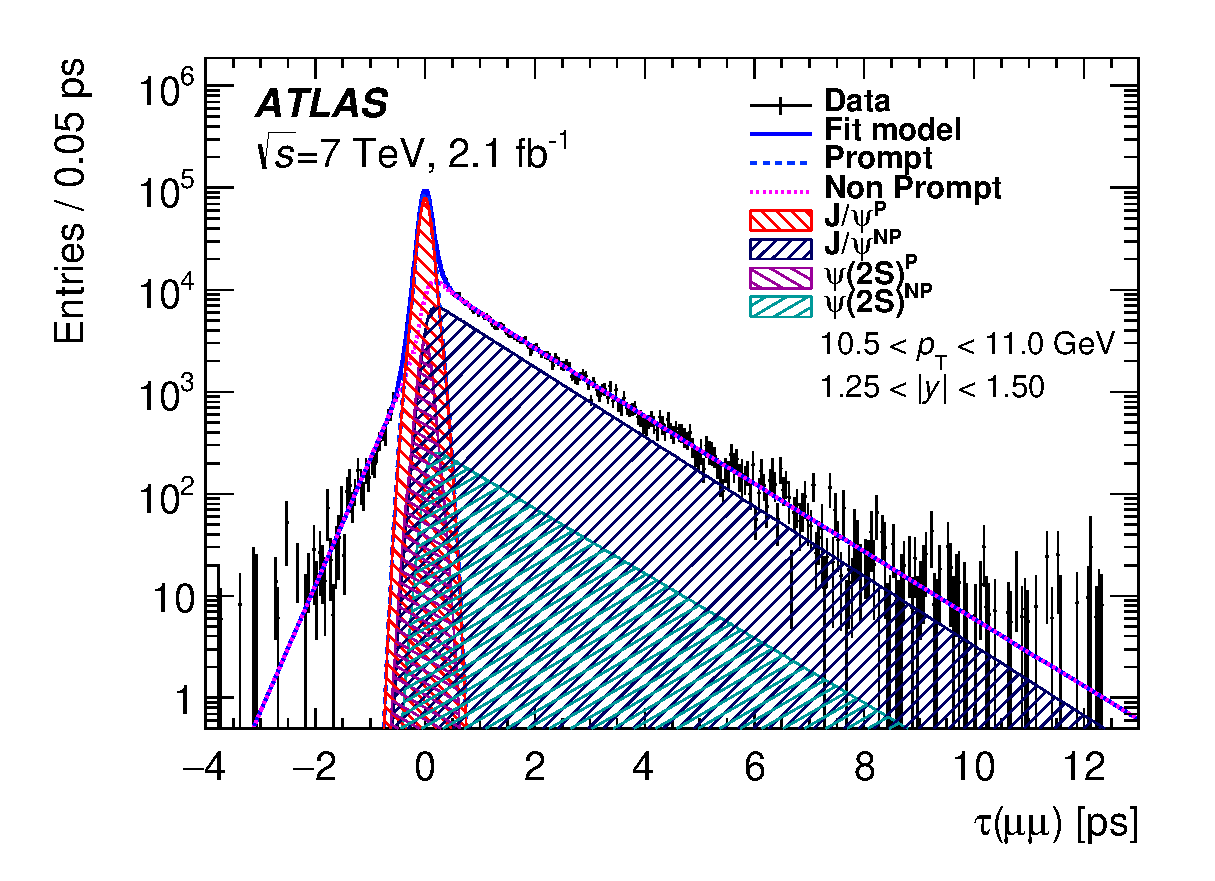
\includegraphics[width=0.51\textwidth]{figures/c_c_Tau_5_5.eps}
      \caption{Projections of the fit result over the mass (left) and pseudo-proper decay time (right) distributions for data collected at $7$~\TeV\  for one typical interval. The data are shown with error bars in black, superimposed with the individual components of the fit result projections, where the total prompt and non-prompt components are represented by the dashed and dotted lines, respectively, and the shaded areas show the signal $\psi$ prompt and non-prompt contributions.\label{fig:fitprojmain}}
  \end{center}
\end{figure} 

\begin{figure} [!ht]
  \begin{center} 
   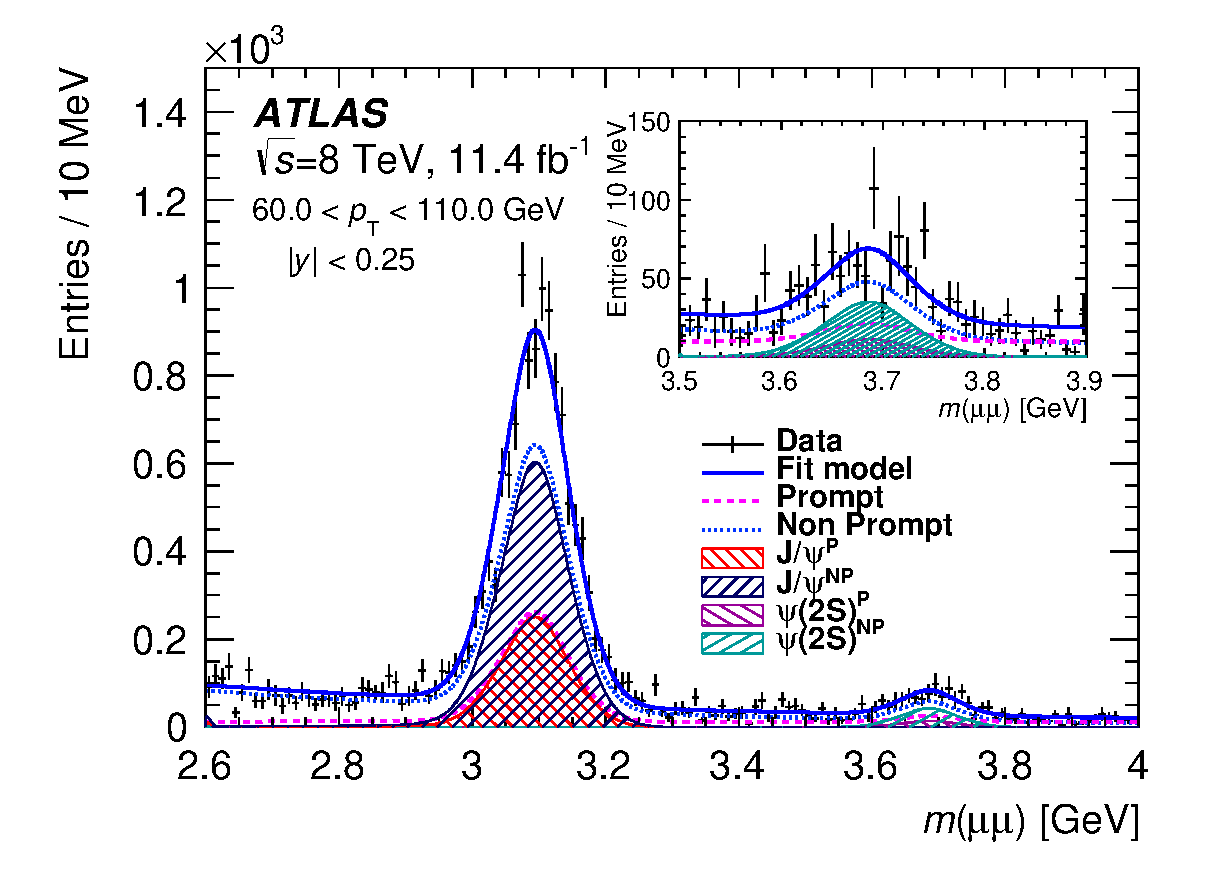
\includegraphics[width=0.51\textwidth]{figures/c_8TeV_c_Mass_23_0.eps}
   \hspace{-0.55cm}
   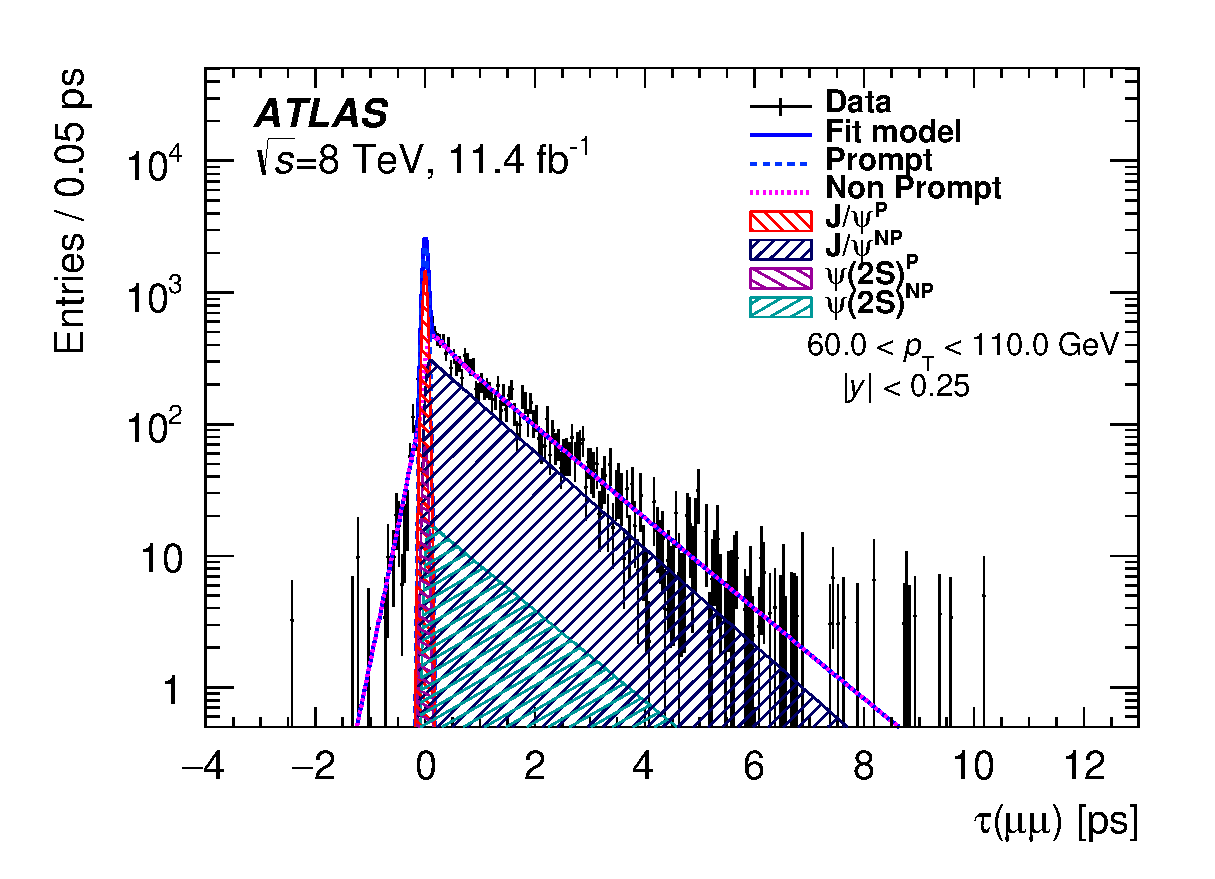
\includegraphics[width=0.51\textwidth]{figures/c_8TeV_c_Tau_23_0.eps}
      \caption{Projections of the fit result over the mass (left) and pseudo-proper decay time (right) distributions for data collected at $8$~\TeV\ for one high-$\pt$ interval. The data are shown with error bars in black, superimposed with the individual components of the fit result projections, where the total prompt and non-prompt components are represented by the dashed and dotted lines, respectively, and the shaded areas show the signal $\psi$ prompt and non-prompt contributions.\label{fig:fitprojmainVIII}}
  \end{center}
\end{figure} 


\subsection{Bin migration corrections}

To account for bin migration effects due to the detector resolution, corrections are applied according to the $\pt$ of the dimuon system.
These corrections are derived from data by comparing analytic functions that are 
fitted to the $\pt$ spectra of dimuon events with and without
convolution by the experimental resolution in $\pt$ (as determined from the fitted mass resolution and measured muon angular resolutions), 
as described in Ref.~\cite{Aad2012dlq}.

The numbers of acceptance- and efficiency-corrected dimuon decays extracted from
the fits in each $\pT$ and rapidity interval are corrected for the differences
between the true and reconstructed values of the dimuon $\pt$.
The correction factors applied to the fitted yields deviate from unity by no more than $1.5\%$, and for the majority of slices are smaller than $1\%$.
The ratio measurement and non-prompt fractions are corrected by the corresponding ratios of
bin migration correction factors.
Using a similar technique, bin migration corrections as a function of $|y|$ are found 
to differ from unity by negligible amounts.
